\documentclass[tikz, crop, margin=2mm]{standalone}

\usepackage{amssymb}

\usetikzlibrary{shapes}
\colorlet{dkgreen}{green!50!black}
\colorlet{dkcyan}{cyan!60!black}

\begin{document}
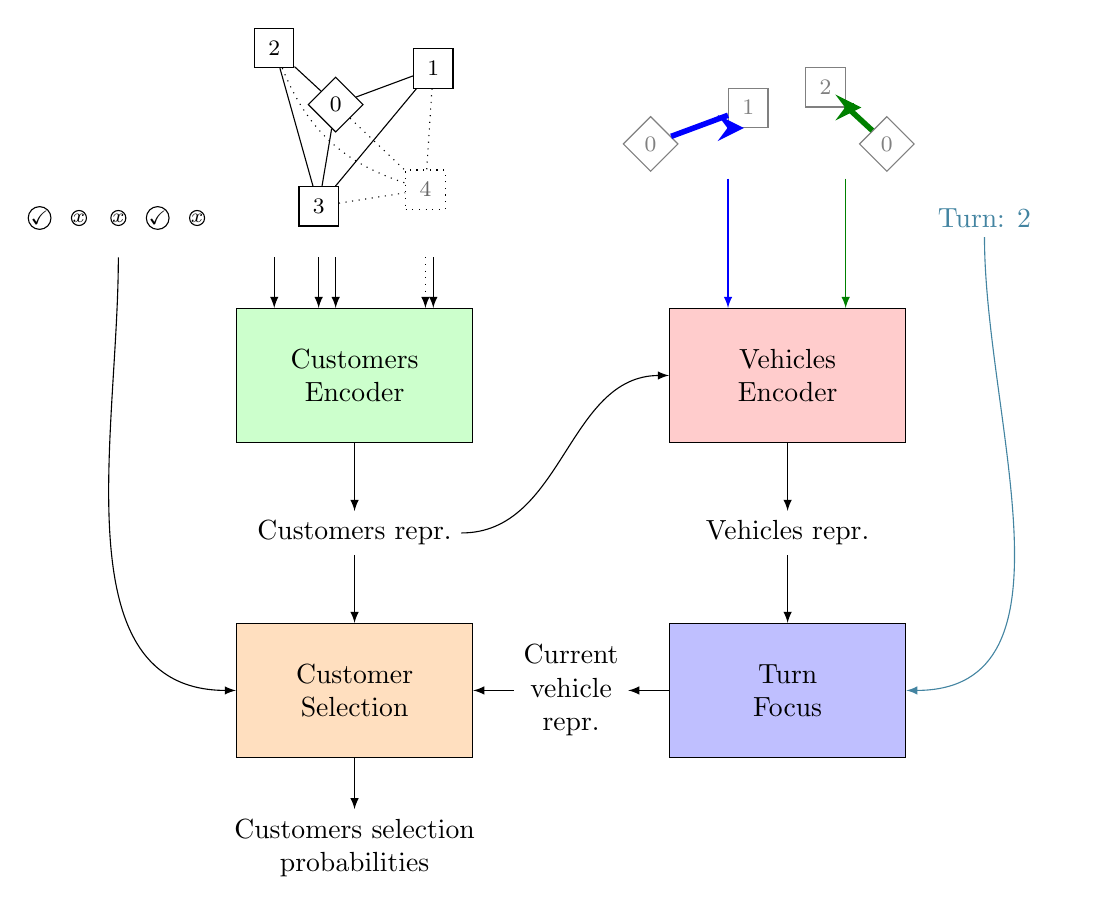
\begin{tikzpicture}[
    depot/.style = {draw, diamond, fill=white, minimum size=7mm, inner sep=1pt, font=\footnotesize},
    cust/.style = {draw, fill=white, minimum size=5mm, inner sep=1pt, font=\footnotesize},
    dyn cust/.style = {dotted, text=black!60, cust},
    cust valid/.style = {draw, circle, fill=white, inner sep=0pt, font=\scriptsize},
    veh/.style = {draw, dart, fill=white, inner sep=1pt, font=\scriptsize}]
    \begin{scope}[shift={(-4,-2.5)}, x={(4mm,0)}, y={(0,4mm)}]
        \node[depot] (depot) at (-0.6,-0.15) {$0$};
        \node[cust] (cust1) at (2.5,1) {$1$};
        \node[cust] (cust2) at (-2.55,1.65) {$2$};
        \node[cust] (cust3) at (-1.14,-3.38) {$3$};
        \node[dyn cust] (cust4) at (2.25,-2.85) {$4$};

        \draw[dotted] (depot) -- (cust4);
        \draw[dotted] (cust1) -- (cust4);
        \draw[dotted] (cust2) to[bend right=25] (cust4);
        \draw[dotted] (cust3) -- (cust4);

        \draw (depot) -- (cust1);
        \draw (depot) -- (cust2);
        \draw (depot) -- (cust3);
        \draw (cust1) -- (cust3);
        \draw (cust2) -- (cust3);
    \end{scope}

    \coordinate (in) at (0,-4.5);
    \node (cust repr) at (-4,-8) {Customers repr.};

    \begin{scope}
        \node[draw, fill=green!20, minimum width=3cm, minimum height=1.7cm, align=center] (cust enc) at (-4,-6) {Customers \\ Encoder};
        \draw[-latex] (in -| depot) -- (cust enc.north -| depot);
        \draw[-latex] (in -| cust1) -- (cust enc.north -| cust1);
        \draw[-latex] (in -| cust2) -- (cust enc.north -| cust2);
        \draw[-latex] (in -| cust3) -- (cust enc.north -| cust3);
        \draw[dotted, -latex] (in -| cust4) -- (cust enc.north -| cust4);
        \draw[-latex] (cust enc) -- (cust repr);
    \end{scope}

    \begin{scope}[shift={(0,-3)}, x={(4mm,0)}, y={(0,4mm)}]
        \node[gray, depot] (depot) at (-0.6,-0.15) {$0$};
        \node[gray, cust] (cust1) at (2.5,1) {$1$};
        
        \draw[blue, line width=3pt, -stealth] (cust1.-135) ++(0.25,0) -- ++(0.25,0);
        \draw[blue, line width=2pt] (depot) -- (cust1);
    \end{scope}

    \begin{scope}[shift={(3,-3)}, x={(4mm,0)}, y={(0,4mm)}]
        \node[gray, depot] (depot) at (-0.6,-0.15) {$0$};
        \node[gray, cust] (cust2) at (-2.55,1.65) {$2$};

        \draw[dkgreen, line width=3pt, -stealth] (cust2.-45) ++(0.25,0) -- ++(0.25,0);
        \draw[dkgreen, line width=2pt] (depot) -- (cust2);
    \end{scope}

    \coordinate (in) at (0,-3.5);

    \node (veh repr) at (1.5,-8) {Vehicles repr.};

    \begin{scope}
        \node[draw, fill=red!20, minimum width=3cm, minimum height=1.7cm, align=center] (veh enc) at (1.5,-6) {Vehicles \\ Encoder};
        \draw[blue, -latex] (in -| cust1.-135) -- (veh enc.north -| cust1.-135);
        \draw[dkgreen, -latex] (in -| cust2.-45) -- (veh enc.north -| cust2.-45);
        \draw[-latex] (cust repr) to[out=0, in=180] (veh enc);
        \draw[-latex] (veh enc) -- (veh repr);
    \end{scope}

    \begin{scope}
        \node[dkcyan] (i2) at (4,-4) {Turn: 2};
    \end{scope}

    \node[align=center] (cur veh repr) at (-1.25,-10) {Current \\ vehicle \\ repr.};

    \begin{scope}
        \node[draw, fill=blue!25, minimum width=3cm, minimum height=1.7cm, align=center] (turn focus) at (1.5,-10) {Turn \\ Focus};

        \draw[dkcyan, -latex] (i2) to[out=-90, in=0] (turn focus);
        \draw[-latex] (veh repr) -- (turn focus);
        \draw[-latex] (turn focus) -- (cur veh repr);
    \end{scope}

    \begin{scope}
        \node[draw, fill=orange!25, minimum width=3cm, minimum height=1.7cm, align=center] (cust select) at (-4,-10) {Customer \\ Selection};

        \draw[-latex] (cust repr) -- (cust select);
        \draw[-latex] (cur veh repr) -- (cust select);

        \node[align=center] (pi) at (-4,-12) {Customers selection \\ probabilities};
        \draw[-latex] (cust select) -- (pi);
    \end{scope}

    \begin{scope}[shift={(-7,-4)}]
        \node[cust valid] at (-1,0) {$\checkmark$};
        \node[cust valid] at (-0.5,0) {$x$};
        \node[cust valid] at (0,0) {$x$};
        \node[cust valid] at (0.5,0) {$\checkmark$};
        \node[cust valid] at (1,0) {$x$};

        \draw[-latex] (0,-0.5) to[out=-90, in=-180] (cust select);
    \end{scope}
\end{tikzpicture}
\end{document}